\chapter{Variación genética y enfermedad}\label{ch:g11:genes-and-disease}

Una pareja con una salud perfecta tiene un primer hijo que, desde las
primeras semanas, tose, no gana peso y tiene un sudor tan salado que un
beso en la frente sabe a sal. El diagnóstico es fibrosis quística: los
dos padres, sin saberlo, llevaban una copia no funcional del mismo \omterm{def:g10:universal-dna:gene}{gen},
y el niño recibió las dos. Una de cada veinticinco personas de
ascendencia europea es \omterm{def:g11:genes-and-disease:genetic}{portadora}; a los padres se les podría haber
dicho, antes del embarazo, con un análisis de una gota de sangre. Este
capítulo trata de las enfermedades escritas en los \omterm{def:g10:universal-dna:gene}{alelos}: cómo se
heredan, cómo se calcula el riesgo a partir de un \omterm{def:g11:genes-and-disease:pedigree}{árbol genealógico},
cómo lee un laboratorio el \omterm{def:g10:universal-dna:gene}{gen} y por qué casi todas las enfermedades
frecuentes son solo en parte genéticas.

\section{Enfermedades de un solo gen}

\begin{definition}[Enfermedad genética, dominante y recesiva]\label{def:g11:genes-and-disease:genetic}
Una \emph{enfermedad genética}\index{enfermedad genética} es una
enfermedad causada por uno o varios \omterm{def:g10:universal-dna:gene}{alelos} mutantes. En una enfermedad
de un solo \omterm{def:g10:universal-dna:gene}{gen}, un \omterm{def:g10:universal-dna:gene}{alelo} es \emph{recesivo}\index{recesivo} si la
enfermedad solo aparece en quienes llevan dos copias de él --- quien
lleva una sola es un \emph{portador}\index{portador} sano --- y
\emph{dominante}\index{dominante} si basta con una copia. Por convenio,
los \omterm{def:g10:universal-dna:gene}{alelos} de un \omterm{def:g10:universal-dna:gene}{gen} se escriben con una letra: $A$ para el \omterm{def:g10:universal-dna:gene}{alelo}
corriente y $a$ para uno mutante recesivo, de modo que un portador es
$Aa$ y una persona afectada es $aa$.
\end{definition}

\begin{example}[La fibrosis quística]\label{ex:g11:genes-and-disease:cf}
El \omterm{def:g10:universal-dna:gene}{gen} CFTR codifica una \omterm{def:g11:gene-expression:protein}{proteína} que deja pasar iones cloruro a través
de la membrana de las \omterm{def:g10:cells-common-unit:cell}{células} que revisten las vías respiratorias, el
tubo digestivo y las glándulas sudoríparas. Al \omterm{def:g10:universal-dna:gene}{alelo} mutante más
frecuente le faltan tres \omterm{def:g10:universal-dna:nucleotide}{nucleótidos} y, por tanto, un \omterm{def:g10:chemistry-of-life:families}{aminoácido}; la
\omterm{def:g11:gene-expression:protein}{proteína} se pliega mal y se destruye. Sin ella, el moco de las vías
respiratorias es espeso y pegajoso, las infecciones se instalan en los
pulmones y los conductos del páncreas se obstruyen. La enfermedad es
\omterm{def:g11:genes-and-disease:genetic}{recesiva}: alrededor de un europeo de cada 25 es \omterm{def:g11:genes-and-disease:genetic}{portador} sano, y un
recién nacido de cada 2500 está afectado. La drepanocitosis
(\cref{ch:g11:enzymes-and-phenotype}) es asimismo \omterm{def:g11:genes-and-disease:genetic}{recesiva}; la
enfermedad de Huntington, una degeneración del cerebro que empieza
hacia los cuarenta, es \omterm{def:g11:genes-and-disease:genetic}{dominante} --- basta un \omterm{def:g10:universal-dna:gene}{alelo} mutante, y toda
persona afectada tuvo un progenitor afectado.
\end{example}

\begin{proposition}[Transmisión de una enfermedad recesiva]\label{prop:g11:genes-and-disease:recessive}
Cada progenitor pasa a cada hijo uno de sus dos \omterm{def:g10:universal-dna:gene}{alelos}, elegido al
azar. Dos \omterm{def:g11:genes-and-disease:genetic}{portadores} $Aa \times Aa$ tienen, por tanto, para cada hijo,
una probabilidad de $1/4$ de un hijo afectado $aa$, de $1/2$ de un
\omterm{def:g11:genes-and-disease:genetic}{portador} $Aa$ y de $1/4$ de un no \omterm{def:g11:genes-and-disease:genetic}{portador} $AA$. Un \omterm{def:g11:genes-and-disease:genetic}{portador} y un no
\omterm{def:g11:genes-and-disease:genetic}{portador} $Aa \times AA$ no tienen ningún hijo afectado y una
probabilidad de uno entre dos de un \omterm{def:g11:genes-and-disease:genetic}{portador}. Una persona afectada y un
no \omterm{def:g11:genes-and-disease:genetic}{portador} $aa \times AA$ solo tienen hijos \omterm{def:g11:genes-and-disease:genetic}{portadores}.
\end{proposition}
\admitted

\begin{omfigure}
\begin{tikzpicture}[font=\small]
  \draw[thick] (0,0) grid[step=1.6] (3.2,3.2);
  \node[anchor=south] at (0.8,3.3) {$A$}; \node[anchor=south] at (2.4,3.3) {$A$};
  \node[anchor=east] at (-0.15,2.4) {$A$}; \node[anchor=east] at (-0.15,0.8) {$a$};
  \node[anchor=south, font=\small\itshape] at (1.6,3.75) {alelo del padre};
  \node[anchor=east, font=\small\itshape, rotate=90] at (-0.65,1.6) {};
  \node[font=\small\itshape, rotate=90, anchor=south] at (-0.75,1.6) {alelo de la madre};
  \node[fill=omDef!15, minimum size=1.5cm] at (0.8,2.4) {$AA$};
  \node[fill=omDef!15, minimum size=1.5cm] at (2.4,2.4) {$AA$};
  \node[fill=omProp!20, minimum size=1.5cm] at (0.8,0.8) {$Aa$};
  \node[fill=omProp!20, minimum size=1.5cm] at (2.4,0.8) {$Aa$};
  \node[anchor=north, align=center] at (1.6,-0.3) {madre portadora $\times$ padre no portador:\\ la mitad de los hijos portadores, ninguno afectado};
  \begin{scope}[xshift=9.6cm]
    \draw[thick] (0,0) grid[step=1.6] (3.2,3.2);
    \node[anchor=south] at (0.8,3.3) {$A$}; \node[anchor=south] at (2.4,3.3) {$a$};
    \node[anchor=east] at (-0.15,2.4) {$A$}; \node[anchor=east] at (-0.15,0.8) {$a$};
    \node[fill=omDef!15, minimum size=1.5cm] at (0.8,2.4) {$AA$};
    \node[fill=omProp!20, minimum size=1.5cm] at (2.4,2.4) {$Aa$};
    \node[fill=omProp!20, minimum size=1.5cm] at (0.8,0.8) {$Aa$};
    \node[fill=omThm!25, minimum size=1.5cm] at (2.4,0.8) {$aa$};
    \node[anchor=north, align=center] at (1.6,-0.3) {dos portadores: $1/4$ afectados,\\ $1/2$ portadores, $1/4$ no portadores};
  \end{scope}
\end{tikzpicture}

{\small Cuadros de Punnett. Cada casilla es una combinación igualmente
probable del \omterm{def:g10:universal-dna:gene}{alelo} de la madre (fila) y del padre (columna). Las
proporciones son probabilidades para cada hijo, no una garantía sobre
cuatro hijos.}
\end{omfigure}

\begin{omfigure}
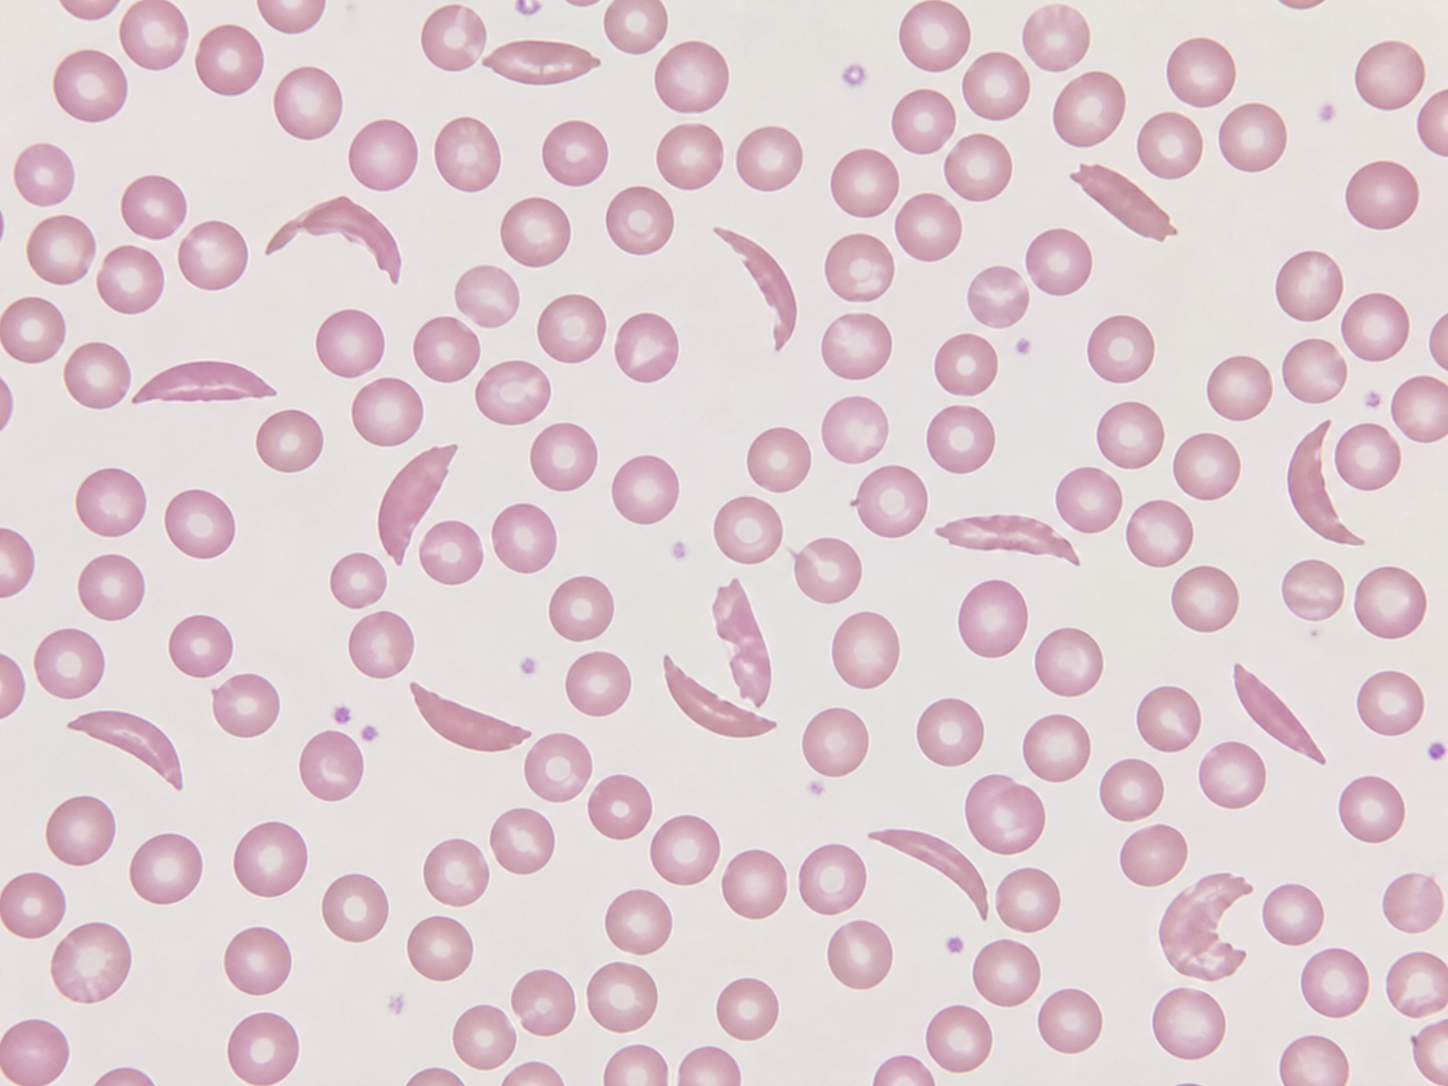
\includegraphics[width=0.56\linewidth]{images/book2/ai/g11-disease-sickle-smear.png}

{\small Un frotis de sangre de una persona con drepanocitosis: glóbulos
rojos redondos y, entre ellos, las medias lunas. El \omterm{def:g11:enzymes-and-phenotype:phenotype}{fenotipo} celular de
una sola sustitución de \omterm{def:g10:chemistry-of-life:families}{aminoácido}, llevada en los dos \omterm{def:g10:universal-dna:gene}{alelos}.}
\end{omfigure}

\section{Leer un árbol genealógico}

\begin{definition}[Árbol genealógico]\label{def:g11:genes-and-disease:pedigree}
Un \emph{árbol genealógico}\index{árbol genealógico} es un diagrama de
una familia a lo largo de varias generaciones: cuadrados para los
varones, círculos para las mujeres, una línea horizontal que une a una
pareja, una línea vertical que baja hasta sus hijos y símbolos
rellenos para las personas afectadas. Las generaciones se numeran I,
II, III desde arriba; los individuos se numeran desde la izquierda.
\end{definition}

\begin{omfigure}
\begin{tikzpicture}[font=\small, line cap=round]
  \tikzset{m/.style={draw, thick, minimum size=0.5cm, inner sep=0},
           f/.style={draw, thick, circle, minimum size=0.5cm, inner sep=0},
           aff/.style={fill=omThm!70}}
  % generation I
  \node[m] (I1) at (2,3) {}; \node[f] (I2) at (3.2,3) {};
  \node[m] (I3) at (6.4,3) {}; \node[f] (I4) at (7.6,3) {};
  \draw[thick] (I1) -- (I2); \draw[thick] (I3) -- (I4);
  \node[anchor=east] at (0.8,3) {I};
  \foreach \n/\x in {1/2, 2/3.2, 3/6.4, 4/7.6} \node[font=\scriptsize, anchor=south] at (\x,3.35) {\n};
  % generation II
  \draw[thick] (2.6,3) -- (2.6,2.3) -- (4.4,2.3); \draw[thick] (1.6,2.3) -- (2.6,2.3);
  \draw[thick] (7.0,3) -- (7.0,2.3) -- (5.6,2.3); \draw[thick] (7.0,2.3) -- (8.4,2.3);
  \node[f] (II1) at (1.6,1.7) {}; \node[m, aff] (II2) at (2.6,1.7) {}; \node[m] (II3) at (4.4,1.7) {};
  \node[f] (II4) at (5.6,1.7) {}; \node[f] (II5) at (7.0,1.7) {}; \node[m] (II6) at (8.4,1.7) {};
  \foreach \x in {1.6,2.6,4.4,5.6,7.0,8.4} \draw[thick] (\x,2.3) -- (\x,1.95);
  \draw[thick] (II3) -- (II4);
  \node[anchor=east] at (0.8,1.7) {II};
  \foreach \n/\x in {1/1.6, 2/2.6, 3/4.4, 4/5.6, 5/7.0, 6/8.4} \node[font=\scriptsize, anchor=north] at (\x,1.42) {\n};
  % generation III
  \draw[thick] (5.0,1.7) -- (5.0,1.0) -- (5.8,1.0); \draw[thick] (4.2,1.0) -- (5.0,1.0);
  \node[m] (III1) at (4.2,0.4) {}; \node[f, aff] (III2) at (5.8,0.4) {};
  \foreach \x in {4.2,5.8} \draw[thick] (\x,1.0) -- (\x,0.65);
  \node[anchor=east] at (0.8,0.4) {III};
  \foreach \n/\x in {1/4.2, 2/5.8} \node[font=\scriptsize, anchor=north] at (\x,0.12) {\n};
  % legend
  \node[m] at (10.2,2.6) {}; \node[anchor=west] at (10.5,2.6) {varón};
  \node[f] at (10.2,1.9) {}; \node[anchor=west] at (10.5,1.9) {mujer};
  \node[m, aff] at (10.2,1.2) {}; \node[anchor=west] at (10.5,1.2) {afectado};
\end{tikzpicture}

{\small Un \omterm{def:g11:genes-and-disease:pedigree}{árbol genealógico} de fibrosis quística. II-2 y III-2 están
afectados; sus padres están sanos. Las dos parejas I-1/I-2 y II-3/II-4
tienen que ser \omterm{def:g11:genes-and-disease:genetic}{portadoras}; II-3, hermano sano de un hijo afectado, es
\omterm{def:g11:genes-and-disease:genetic}{portador} con probabilidad $2/3$.}
\end{omfigure}

\begin{method}[Analizar un árbol genealógico]\label{met:g11:genes-and-disease:analyse}
\begin{enumerate}
  \item \emph{¿\omterm{def:g11:genes-and-disease:genetic}{Dominante} o \omterm{def:g11:genes-and-disease:genetic}{recesiva}?} Un hijo afectado de dos padres
        sanos significa \omterm{def:g11:genes-and-disease:genetic}{recesiva} (los padres son \omterm{def:g11:genes-and-disease:genetic}{portadores}). Una
        persona afectada con un progenitor afectado en todas las
        generaciones sugiere \omterm{def:g11:genes-and-disease:genetic}{dominante}.
  \item \emph{¿En un \omterm{def:g11:cell-cycle-mitosis:chromosome}{cromosoma} sexual?} Si solo hay varones afectados y
        también lo están los hermanos o el padre de sus madres,
        sospecha del \omterm{def:g11:cell-cycle-mitosis:chromosome}{cromosoma} X (más abajo). Si no, el \omterm{def:g10:universal-dna:gene}{gen} está en un
        \omterm{def:g11:cell-cycle-mitosis:chromosome}{cromosoma} corriente.
  \item \emph{Asigna \omterm{def:g11:enzymes-and-phenotype:phenotype}{genotipos}}: en una enfermedad \omterm{def:g11:genes-and-disease:genetic}{recesiva}, las
        personas afectadas son $aa$; sus padres y sus hijos llevan al
        menos un $a$; los hermanos sanos de una persona afectada son
        $AA$ o $Aa$.
  \item \emph{Calcula el riesgo} de un hijo previsto combinando los
        \omterm{def:g11:enzymes-and-phenotype:phenotype}{genotipos} de los padres en un cuadro de Punnett; cuando el
        \omterm{def:g11:enzymes-and-phenotype:phenotype}{genotipo} de un progenitor es incierto, pondera cada
        posibilidad por su probabilidad.
\end{enumerate}
\end{method}

\begin{example}[Los dos tercios]\label{ex:g11:genes-and-disease:twothirds}
¿Por qué un hermano sano de un hijo afectado es \omterm{def:g11:genes-and-disease:genetic}{portador} con
probabilidad $2/3$ y no $1/2$? Los padres son $Aa \times Aa$; un hijo
es $AA$, $Aa$, $aA$ o $aa$ con la misma probabilidad. Saber que está
sano descarta $aa$: quedan tres casos, de los que dos son \omterm{def:g11:genes-and-disease:genetic}{portadores}.
Si se casa con una mujer de la población general (\omterm{def:g11:genes-and-disease:genetic}{portadora} con
probabilidad $1/25$), el riesgo de un primer hijo afectado es
$2/3 \times 1/25 \times 1/4 = 1/150$.
\end{example}

\section{Genes del cromosoma X}

\begin{proposition}[Herencia ligada al X]\label{prop:g11:genes-and-disease:xlinked}
Las mujeres llevan dos \omterm{def:g10:universal-dna:information}{cromosomas} X, y los varones un X y un Y. Un
\omterm{def:g10:universal-dna:gene}{alelo} \omterm{def:g11:genes-and-disease:genetic}{recesivo} del \omterm{def:g11:cell-cycle-mitosis:chromosome}{cromosoma} X queda enmascarado en una mujer por su
segundo X, pero un varón, que no tiene segundo X, lo expresa. Una
enfermedad así afecta por tanto sobre todo a los varones; las hijas de
un varón afectado son todas \omterm{def:g11:genes-and-disease:genetic}{portadoras}; una madre \omterm{def:g11:genes-and-disease:genetic}{portadora} pasa el
\omterm{def:g10:universal-dna:gene}{alelo} a la mitad de sus hijos varones, que están afectados, y a la
mitad de sus hijas, que son \omterm{def:g11:genes-and-disease:genetic}{portadoras}. La hemofilia, en la que la
sangre no coagula, es el ejemplo clásico; el daltonismo para el rojo y
el verde (\cref{ch:g11:the-eye}) es otro.
\end{proposition}
\admitted

\begin{omfigure}
\begin{tikzpicture}[font=\small]
  \draw[thick] (0,0) grid[step=2.2] (4.4,4.4);
  \node[anchor=south] at (1.1,4.5) {$X^H$}; \node[anchor=south] at (3.3,4.5) {$Y$};
  \node[anchor=east] at (-0.15,3.3) {$X^H$}; \node[anchor=east] at (-0.15,1.1) {$X^h$};
  \node[anchor=south, font=\small\itshape] at (2.2,5.0) {padre (sano)};
  \node[font=\small\itshape, rotate=90, anchor=south] at (-0.95,2.2) {madre (portadora)};
  \node[fill=omDef!15, minimum size=2.1cm, align=center, font=\footnotesize] at (1.1,3.3) {$X^HX^H$\\ niña sana};
  \node[fill=omDef!15, minimum size=2.1cm, align=center, font=\footnotesize] at (3.3,3.3) {$X^HY$\\ niño sano};
  \node[fill=omProp!20, minimum size=2.1cm, align=center, font=\footnotesize] at (1.1,1.1) {$X^HX^h$\\ niña portadora};
  \node[fill=omThm!25, minimum size=2.1cm, align=center, font=\footnotesize] at (3.3,1.1) {$X^hY$\\ niño afectado};
  \node[anchor=west, align=left, text width=6cm] at (5.4,2.2) {Una madre portadora y un padre sano: la mitad de los hijos varones afectados, la mitad de las hijas portadoras y ninguna hija afectada. El $Y$ no lleva ninguna copia del gen, así que la única copia de un hijo varón viene de su madre.};
\end{tikzpicture}

{\small Cuadro de Punnett de una enfermedad \omterm{def:g11:genes-and-disease:genetic}{recesiva} ligada al X, como
la hemofilia ($h$, el \omterm{def:g10:universal-dna:gene}{alelo} mutante; $H$, el corriente).}
\end{omfigure}

\section{Leer el gen mismo}

\begin{proposition}[Pruebas genéticas]\label{prop:g11:genes-and-disease:testing}
Los \omterm{def:g10:universal-dna:gene}{alelos} que lleva una persona pueden leerse directamente en su \omterm{def:g10:universal-dna:information}{ADN},
extraído de unas pocas \omterm{def:g10:cells-common-unit:cell}{células} (sangre, saliva y, para un feto, una
muestra de la placenta o del líquido que lo rodea). La región del \omterm{def:g10:universal-dna:gene}{gen}
se copia millones de veces mediante una reacción que imita la
replicación (\cref{ch:g11:dna-replication}) en un tubo de ensayo, y
después o bien se secuencia, o bien se corta con \omterm{def:g11:enzymes-and-phenotype:enzyme}{enzimas} que reconocen
secuencias concretas y se separa por tamaños en un gel: un \omterm{def:g10:universal-dna:gene}{alelo}
mutante que haya ganado, perdido o cambiado un sitio de corte da
fragmentos de longitudes distintas, visibles como bandas. Estas
pruebas identifican \omterm{def:g11:genes-and-disease:genetic}{portadores} antes de concebir un hijo, diagnostican
a un feto y detectan la \omterm{def:g11:mutations:mutation}{mutación} en un recién nacido antes de que
aparezcan los síntomas.
\end{proposition}
\admitted

\begin{omfigure}
\begin{tikzpicture}[font=\small]
  % gel: 4 lanes
  \fill[gray!15] (0,0) rectangle (7.2,4.2);
  \foreach \x/\l in {0.9/{marcador de\\ tamaños}, 2.7/{$AA$}, 4.5/{$Aa$}, 6.3/{$aa$}} \node[anchor=south, align=center] at (\x,4.3) {\l};
  % ladder
  \foreach \y in {3.6,3.1,2.6,2.0,1.4,0.8} \fill[omDef!70] (0.5,\y) rectangle (1.3,\y+0.1);
  % AA: one band (600 bp, cut into 400+200? keep: A allele = one long fragment at 3.1)
  \fill[omThm!80] (2.3,3.1) rectangle (3.1,3.2);
  % Aa: long fragment + two short
  \fill[omThm!80] (4.1,3.1) rectangle (4.9,3.2);
  \fill[omThm!80] (4.1,2.0) rectangle (4.9,2.1);
  \fill[omThm!80] (4.1,1.4) rectangle (4.9,1.5);
  % aa: two short only
  \fill[omThm!80] (5.9,2.0) rectangle (6.7,2.1);
  \fill[omThm!80] (5.9,1.4) rectangle (6.7,1.5);
  \draw[->, thick] (7.6,3.8) -- (7.6,0.8) node[midway, right, align=left] {sentido de la\\ migración:\\ los fragmentos pequeños\\ avanzan más};
  \node[anchor=east, font=\scriptsize] at (0.4,3.15) {600 pb};
  \node[anchor=east, font=\scriptsize] at (0.4,2.05) {400 pb};
  \node[anchor=east, font=\scriptsize] at (0.4,1.45) {200 pb};
\end{tikzpicture}

{\small Leer \omterm{def:g10:universal-dna:gene}{alelos} en un gel. El \omterm{def:g10:universal-dna:gene}{alelo} mutante $a$ ha ganado un sitio
de corte: el fragmento de 600 pares de \omterm{def:g10:universal-dna:nucleotide}{bases} de $A$ queda cortado en
400 y 200. Un \omterm{def:g11:genes-and-disease:genetic}{portador} muestra las tres bandas; una persona afectada,
solo las dos cortas.}
\end{omfigure}

\begin{omfigure}
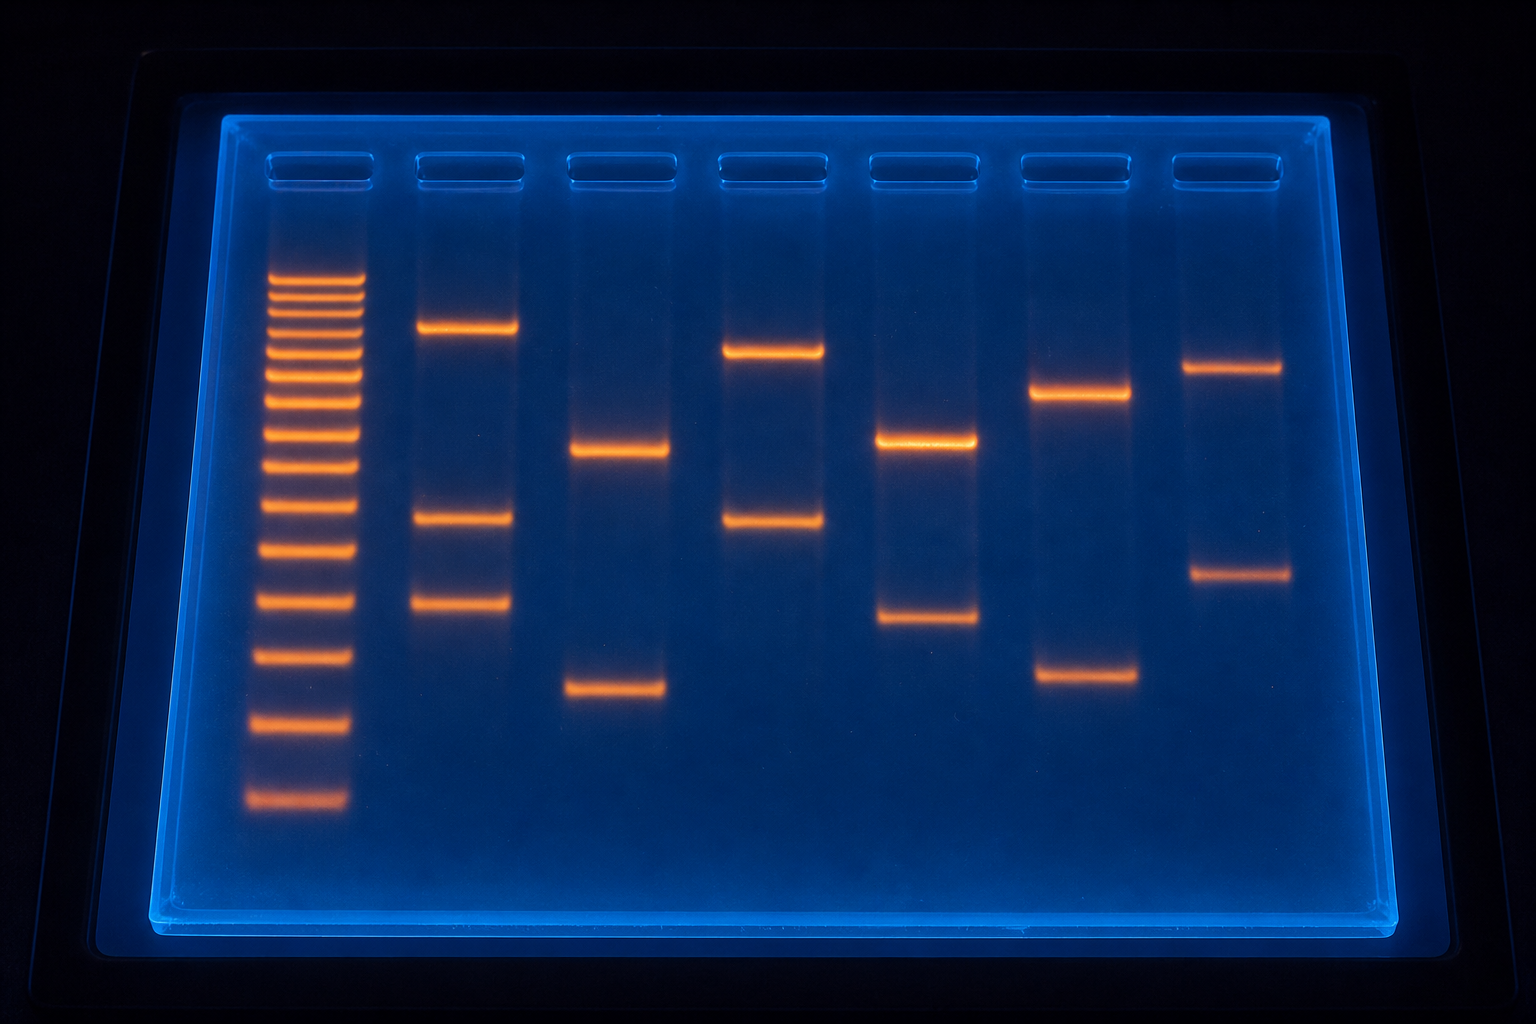
\includegraphics[width=0.56\linewidth]{images/book2/ai/g11-disease-gel.png}

{\small Un gel de electroforesis bajo luz ultravioleta: fragmentos de
\omterm{def:g10:universal-dna:information}{ADN}, teñidos con un colorante fluorescente, ordenados por longitud.
Cada calle es una muestra; el patrón de bandas lee los \omterm{def:g10:universal-dna:gene}{alelos}.}
\end{omfigure}

\begin{example}[Qué puede y qué no puede decir una prueba]\label{ex:g11:genes-and-disease:testsays}
Una prueba de \omterm{def:g11:genes-and-disease:genetic}{portadores} de fibrosis quística busca los cincuenta
\omterm{def:g10:universal-dna:gene}{alelos} mutantes más frecuentes y encuentra alrededor del 90\% de los
\omterm{def:g11:genes-and-disease:genetic}{portadores}: un resultado negativo baja la probabilidad de ser \omterm{def:g11:genes-and-disease:genetic}{portador}
de $1/25$ a alrededor de $1/250$, pero no la anula. Un diagnóstico
prenatal en el feto de dos \omterm{def:g11:genes-and-disease:genetic}{portadores} conocidos es casi seguro, y
enfrenta a los padres a una decisión que la biología no toma por ellos.
Una prueba de la enfermedad de Huntington le dice a una persona sana de
treinta años si la enfermedad llegará; un tercio de quienes tienen
derecho a ella eligen no saberlo.
\end{example}

\section{Enfermedades de muchos genes y de un modo de vida}

\begin{proposition}[Enfermedades multifactoriales]\label{prop:g11:genes-and-disease:multifactorial}
Casi todas las enfermedades frecuentes --- la diabetes de tipo 2, las
enfermedades del corazón y de las arterias, la mayoría de los cánceres,
el asma --- son
\emph{multifactoriales}\index{enfermedad multifactorial}: decenas o
cientos de \omterm{def:g10:universal-dna:gene}{alelos} desplazan cada uno un poco el riesgo, y el ambiente
(dieta, actividad, tabaco, infecciones) lo desplaza mucho. Una
enfermedad así aparece en familias sin seguir las reglas de un solo
\omterm{def:g10:universal-dna:gene}{gen}, y una predisposición genética es un riesgo, no una condena: los
mismos \omterm{def:g10:universal-dna:gene}{alelos} producen enfermedad con un modo de vida y no con otro.
\end{proposition}
\begin{proof}[Pruebas experimentales]
Los gemelos idénticos comparten todos sus \omterm{def:g10:universal-dna:gene}{alelos}; cuando uno tiene
diabetes de tipo 2, el otro la tiene en alrededor del 70\% de los casos
--- muy por encima del 8\% de la población, así que los \omterm{def:g10:universal-dna:gene}{genes} importan
--- pero no en el 100\%, así que los \omterm{def:g10:universal-dna:gene}{genes} no deciden. Las poblaciones
que pasaron en una generación de una dieta rural a otra urbana vieron
multiplicarse varias veces la enfermedad con los mismos \omterm{def:g10:universal-dna:gene}{genes}. Entre
las personas que llevan muchos \omterm{def:g10:universal-dna:gene}{alelos} de riesgo, quienes se mantienen
activas y delgadas desarrollan la enfermedad a una fracción del ritmo
de quienes no lo hacen.
\end{proof}

\begin{omfigure}
\begin{tikzpicture}
\begin{axis}[
  ybar, bar width=12pt,
  width=0.8\linewidth, height=5.4cm,
  axis x line=bottom, axis y line=left,
  ymin=0, ymax=40, ylabel={diabetes de tipo 2 a los 60 años (\%)},
  ylabel style={font=\small},
  symbolic x coords={pocos alelos de riesgo, media, muchos alelos de riesgo},
  xtick=data, tick label style={font=\small},
  enlarge x limits=0.25, ytick={0,10,20,30,40},
  legend style={at={(0.5,-0.2)}, anchor=north, legend columns=2, font=\small, draw=none},
  nodes near coords, nodes near coords style={font=\scriptsize},
]
\addplot[fill=omMeth!50, draw=omMeth] coordinates {(pocos alelos de riesgo,3) (media,6) (muchos alelos de riesgo,12)};
\addplot[fill=omThm!50, draw=omThm] coordinates {(pocos alelos de riesgo,9) (media,17) (muchos alelos de riesgo,34)};
\legend{activo y delgado, sedentario y con sobrepeso}
\end{axis}
\end{tikzpicture}

{\small Riesgo de diabetes de tipo 2 según la puntuación genética y el
modo de vida (redondeado a partir de estudios de población). Los \omterm{def:g10:universal-dna:gene}{genes}
multiplican el riesgo por cuatro de un extremo a otro de la escala; el
modo de vida lo multiplica por tres en cada punto de la escala. Los dos
actúan juntos.}
\end{omfigure}

\begin{remark}[Qué significa entonces ``genética'']\label{rem:g11:genes-and-disease:meaning}
La fibrosis quística es genética en sentido estricto: el \omterm{def:g11:enzymes-and-phenotype:phenotype}{genotipo}
determina la enfermedad sea cual sea el ambiente, y el ambiente solo
cambia cómo se vive. La diabetes de tipo 2 es genética en un sentido
más débil: el \omterm{def:g11:enzymes-and-phenotype:phenotype}{genotipo} fija una susceptibilidad que el ambiente
realiza o no. Entre ambas están la fenilcetonuria, donde una dieta
anula el efecto del \omterm{def:g11:enzymes-and-phenotype:phenotype}{genotipo}, y el \omterm{def:g11:genes-and-disease:genetic}{portador} de drepanocitosis, cuyo
\omterm{def:g10:universal-dna:gene}{alelo} es una enfermedad en un lugar y una protección en otro.
``¿Es genética?'' rara vez es una pregunta de sí o no; ``¿cuánto y en
qué condiciones?'' es la pregunta que hay que hacer.
\end{remark}

\section{Ejercicios}

\begin{exercise}[$\star$]\label{exo:g11:genes-and-disease:1}
Define \omterm{def:g10:universal-dna:gene}{alelo} \omterm{def:g11:genes-and-disease:genetic}{recesivo}, \omterm{def:g10:universal-dna:gene}{alelo} \omterm{def:g11:genes-and-disease:genetic}{dominante} y \omterm{def:g11:genes-and-disease:genetic}{portador}.
\end{exercise}

\begin{exercise}[$\star$]\label{exo:g11:genes-and-disease:2}
Dos \omterm{def:g11:genes-and-disease:genetic}{portadores} de fibrosis quística tienen un hijo. Da la probabilidad
de que esté afectado, de que sea \omterm{def:g11:genes-and-disease:genetic}{portador} o de que no sea ninguna de
las dos cosas.
\end{exercise}

\begin{exercise}[$\star$]\label{exo:g11:genes-and-disease:3}
En la figura del \omterm{def:g11:genes-and-disease:pedigree}{árbol genealógico}, da los \omterm{def:g11:enzymes-and-phenotype:phenotype}{genotipos} de I-1, I-2, II-2
y III-2.
\end{exercise}

\begin{exercise}[$\star$]\label{exo:g11:genes-and-disease:4}
¿Por qué las enfermedades \omterm{def:g11:genes-and-disease:genetic}{recesivas} ligadas al X son mucho más
frecuentes en los varones?
\end{exercise}

\begin{exercise}[$\star$]\label{exo:g11:genes-and-disease:5}
¿Qué es una \omterm{prop:g11:genes-and-disease:multifactorial}{enfermedad multifactorial}? Da dos ejemplos.
\end{exercise}

\begin{exercise}[$\star\star$]\label{exo:g11:genes-and-disease:6}
Una persona con fibrosis quística se casa con una no \omterm{def:g11:genes-and-disease:genetic}{portadora}. ¿Cómo
son sus hijos? ¿Y los hijos de uno de ellos con una \omterm{def:g11:genes-and-disease:genetic}{portadora}?
\end{exercise}

\begin{exercise}[$\star\star$]\label{exo:g11:genes-and-disease:7}
En la figura del \omterm{def:g11:genes-and-disease:pedigree}{árbol genealógico}, calcula la probabilidad de que II-1
sea \omterm{def:g11:genes-and-disease:genetic}{portadora}, y la probabilidad de que un hijo de II-1 y de un varón
de la población general esté afectado.
\end{exercise}

\begin{exercise}[$\star\star$]\label{exo:g11:genes-and-disease:8}
Un hombre con la enfermedad de Huntington (\omterm{def:g11:genes-and-disease:genetic}{dominante}, un \omterm{def:g10:universal-dna:gene}{alelo} mutante)
y una mujer sana tienen cuatro hijos. ¿Cuál es la probabilidad de que
un hijo dado herede la enfermedad? ¿Y de que no la herede ninguno de
los cuatro?
\end{exercise}

\begin{exercise}[$\star\star$]\label{exo:g11:genes-and-disease:9}
Un hombre hemofílico se casa con una mujer no \omterm{def:g11:genes-and-disease:genetic}{portadora}. Describe los
\omterm{def:g11:enzymes-and-phenotype:phenotype}{genotipos} y los \omterm{def:g11:enzymes-and-phenotype:phenotype}{fenotipos} de sus hijos, y los de los nietos por vía de
una hija casada con un hombre sano.
\end{exercise}

\begin{exercise}[$\star\star$]\label{exo:g11:genes-and-disease:10}
En la figura del gel, ¿qué bandas mostraría una persona que llevara dos
\omterm{def:g10:universal-dna:gene}{alelos} mutantes distintos, uno que añadiera el sitio de corte y otro
que eliminara otros 100 pares de \omterm{def:g10:universal-dna:nucleotide}{bases} del fragmento de 400?
\end{exercise}

\begin{exercise}[$\star\star$]\label{exo:g11:genes-and-disease:11}
Explica por qué la fibrosis quística es mil veces más frecuente en
Europa que en el este de Asia, aunque la tasa de \omterm{def:g11:mutations:mutation}{mutación} sea la misma.
\end{exercise}

\begin{exercise}[$\star\star\star$]\label{exo:g11:genes-and-disease:12}
El primer hijo de una pareja tiene fibrosis quística. Calcula la
probabilidad de que el segundo esté afectado, y después la de que lo
esté al menos uno de los dos siguientes. Explica por qué ``ya hemos
tenido nuestro uno de cada cuatro'' es una falacia.
\end{exercise}

\begin{exercise}[$\star\star\star$]\label{exo:g11:genes-and-disease:13}
Una prueba de \omterm{def:g11:genes-and-disease:genetic}{portadores} detecta el 90\% de los \omterm{def:g10:universal-dna:gene}{alelos} mutantes. Una
mujer de la población general da negativo. Calcula la probabilidad que
le queda de ser \omterm{def:g11:genes-and-disease:genetic}{portadora}, y el riesgo de un hijo afectado con una
pareja que es \omterm{def:g11:genes-and-disease:genetic}{portador} conocido.
\end{exercise}

\begin{exercise}[$\star\star\star$]\label{exo:g11:genes-and-disease:14}
En la figura de la diabetes, compara el efecto de pasar de ``muchos'' a
``pocos'' \omterm{def:g10:universal-dna:gene}{alelos} de riesgo (imposible) con el de pasar de sedentario a
activo (posible), para una persona con muchos \omterm{def:g10:universal-dna:gene}{alelos} de riesgo. ¿Para
qué debería usarse una puntuación de riesgo genético?
\end{exercise}

\begin{exercise}[$\star\star\star$]\label{exo:g11:genes-and-disease:15}
Discute, en un párrafo, qué ofrece y qué cuesta una prueba de la
enfermedad de Huntington a un adulto joven y sano cuyo progenitor está
afectado, y por qué la decisión es suya.
\end{exercise}

\section{Problema: Una familia, un gen}

\begin{problem}[{Problema de fin de semana --- una familia con fibrosis
quística seguida a lo largo de tres generaciones: genotipos asignados,
riesgos calculados para cada hijo previsto, una prueba de laboratorio
leída y la aritmética de una población de portadores}]
\label{pb:g11:genes-and-disease:1}
Lea y Tom, los dos sanos, tienen tres hijos: Max (sano), Zoé (fibrosis
quística) y Lou (sana). Ana, la hermana de Tom, está sana y casada con
Karim, en cuya familia no hay antecedentes de la enfermedad; esperan un
hijo. En la población, una persona de cada 25 es \omterm{def:g11:genes-and-disease:genetic}{portadora}.

\medskip
\noindent\textbf{Parte I --- \omterm{def:g11:enzymes-and-phenotype:phenotype}{Genotipos}.}
\begin{enumerate}
  \item ¿Es la enfermedad \omterm{def:g11:genes-and-disease:genetic}{dominante} o \omterm{def:g11:genes-and-disease:genetic}{recesiva}? Justifícalo a partir de
        la familia.
  \item Da los \omterm{def:g11:enzymes-and-phenotype:phenotype}{genotipos} de Lea, de Tom y de Zoé.
  \item ¿Cuáles son los \omterm{def:g11:enzymes-and-phenotype:phenotype}{genotipos} posibles de Max, y con qué
        probabilidades?
  \item ¿Cuál es la probabilidad de que Ana sea \omterm{def:g11:genes-and-disease:genetic}{portadora}? (Piensa en
        sus padres.)
  \item ¿Cuál es la probabilidad de que Karim sea \omterm{def:g11:genes-and-disease:genetic}{portador}?
\end{enumerate}

\medskip
\noindent\textbf{Parte II --- Riesgos.}
\begin{enumerate}[resume]
  \item Calcula la probabilidad de que el hijo de Ana y Karim esté
        afectado.
  \item Lea y Tom se plantean un cuarto hijo. ¿Probabilidad de que esté
        afectado? ¿Y de que sea \omterm{def:g11:genes-and-disease:genetic}{portador}?
  \item Max, ya adulto, se casa con una mujer de la población general.
        ¿Probabilidad de un primer hijo afectado?
  \item Zoé, ya adulta, se casa con un hombre de la población general.
        ¿Probabilidad de un hijo afectado? ¿Y de un hijo \omterm{def:g11:genes-and-disease:genetic}{portador}?
  \item Lou se casa con un primo hermano, hijo de Ana y Karim. Calcula
        la probabilidad de un hijo afectado. ¿Por qué es mayor que en
        el caso de Max?
\end{enumerate}

\medskip
\noindent\textbf{Parte III --- La prueba.}
El \omterm{def:g10:universal-dna:gene}{alelo} mutante que lleva esta familia añade un sitio de corte: el
\omterm{def:g10:universal-dna:gene}{alelo} corriente da un fragmento de 900 pares de \omterm{def:g10:universal-dna:nucleotide}{bases} y el mutante da
uno de 600 y otro de 300.
\begin{enumerate}[resume]
  \item Dibuja, o describe, las bandas que se esperan para Zoé, para
        Tom y para una persona no \omterm{def:g11:genes-and-disease:genetic}{portadora}.
  \item Se analiza a Max: una sola banda de 900. ¿Cuál es ahora su
        \omterm{def:g11:enzymes-and-phenotype:phenotype}{genotipo}, y el nuevo riesgo para su primer hijo (pregunta 8)?
  \item Se analiza a Ana: bandas de 900, 600 y 300. Vuelve a calcular
        el riesgo para su hijo.
  \item La prueba de Karim no encuentra ninguno de los cincuenta \omterm{def:g10:universal-dna:gene}{alelos}
        mutantes más frecuentes, que cubren el 90\% de los \omterm{def:g11:genes-and-disease:genetic}{portadores}.
        Calcula la probabilidad que le queda de ser \omterm{def:g11:genes-and-disease:genetic}{portador} y vuelve a
        calcular el riesgo.
  \item Una prueba prenatal del feto de Ana y Karim muestra bandas de
        900, 600 y 300. ¿Cuál es el \omterm{def:g11:enzymes-and-phenotype:phenotype}{genotipo} del feto, y su \omterm{def:g11:enzymes-and-phenotype:phenotype}{fenotipo}?
\end{enumerate}

\medskip
\noindent\textbf{Parte IV --- La población.}
\begin{enumerate}[resume]
  \item Si una persona de cada 25 es \omterm{def:g11:genes-and-disease:genetic}{portadora}, ¿cuál es la
        probabilidad de que los dos miembros de una pareja al azar sean
        \omterm{def:g11:genes-and-disease:genetic}{portadores} y, por tanto, la frecuencia de recién nacidos
        afectados?
  \item Compárala con el uno de cada 2500 observado. Coméntalo.
  \item Casi todas las personas afectadas morían antes en la infancia.
        Explica por qué, aun así, el \omterm{def:g10:universal-dna:gene}{alelo} mutante se mantuvo en una
        frecuencia de una copia de cada 50, usando el número de copias
        que llevan los \omterm{def:g11:genes-and-disease:genetic}{portadores} sanos frente a las personas
        afectadas.
  \item Los tratamientos permiten hoy que casi todas las personas
        afectadas lleguen a la edad adulta y tengan hijos. Predice el
        efecto sobre la frecuencia del \omterm{def:g10:universal-dna:gene}{alelo} en las generaciones
        venideras, y su magnitud.
  \item Enuncia el resultado: el uno de cada cuatro de dos \omterm{def:g11:genes-and-disease:genetic}{portadores},
        los dos de cada tres de un hermano sano y lo que el gel añadió
        a la aritmética de esta familia.
\end{enumerate}
\end{problem}
